\section{System design}
\label{s:system}

The verified artifact of this paper is \txn, a Go package that gives clients an
abstraction of a disk with crash-safe writes. This section aims to convey what
the journal is, why its implementation deserves verification, and how systems can be built
using it. First, \autoref{s:system:api} explains how a developer uses
\txn to write a concurrent storage system, informally laying out what the
package's requirements and guarantees are. Then,
\autoref{s:system:impl} explains how the journal is implemented.
% Finally, \autoref{sec:overview} lays out the verification methodology for
% \txn and applications built on top of it.

% Later sections
% give the formal specification~(\autoref{s:design}) and interesting details of
% the proof~(\autoref{s:proof}).

\subsection{Programming with \txn}
\label{s:system:api}

Developers use the journal to turn several storage operations into an atomic journal operation that commits to disk using the \txn
interface listed in \autoref{fig:buftxn}.  \cc{Begin} starts a
journal operation, returning a \cc{*Op} object, which keeps track of the
objects read or written in the operation.  An object is addressed by the
\cc{Addr} struct, which names a block address and bit offset within the block. \simplenfs
has objects for on-disk blocks and on-disk inodes, while the
complete NFS server also uses objects for individual allocator bits.

\cc{ReadBuf} reads an object into an in-memory \cc{*Buf} struct, returning the latest value of the
object within this journal operation.  If the operation hasn't read the
object yet, it reads the latest value from disk (or from a recently
committed operation).  A journal operation can modify the returned buffer in place and
then mark the buffer as dirty with \cc{SetDirty}. To overwrite an object without
reading it the application can call \cc{OverWrite}. When the operation is
fully prepared, the application commits it atomically using \cc{Commit}; setting
\cc{wait=true} additionally forces the journal to flush the results to disk.
In either case the writes in the operation appear together on disk or not at
all even if the system crashes. The application can also call \cc{Flush} to
make the journal persist several committed but unstable operations to disk.

While \txn provides crash-safe atomic updates to disk with this interface, it is the developer's job
to provide concurrency control to prevent concurrent operations from manipulating
the same on-disk objects. In a file system a common strategy for concurrency
control is to use a per-file lock that protects both the file metadata and any
data blocks associated with the file, and this strategy is the one
used by \gnfs and \simplenfs.
To make it easier for a file system to maintain these locks,
\txn includes a lockmap library that behaves as if it were a large array of
locks but with a more memory-efficient implementation; the
Guava Striped documentation describes the idea well~\cite{guava-striped}.
%which in \gnfs
%and \simplenfs is used to lock files by inode number.


\begin{figure}
  \begin{Verbatim}[commandchars=\\\{\},numbers=left,firstnumber=1,stepnumber=1,codes={\catcode`\$=3\catcode`\^=7\catcode`\_=8},fontsize=\small,numbersep=6pt,xleftmargin=0.2in]
\PY{k+kd}{func} \PY{n+nx}{NFS3\PYZus{}WRITE}\PY{p}{(}\PY{n+nx}{args} \PY{n+nx}{WRITE3args}\PY{p}{)} \PY{n+nx}{WRITE3res} \PY{p}{\PYZob{}}
  \PY{n+nx}{inum} \PY{o}{:=} \PY{n+nx}{fh2ino}\PY{p}{(}\PY{n+nx}{args}\PY{p}{.}\PY{n+nx}{File}\PY{p}{)}
  \PY{k}{if} \PY{p}{!}\PY{n+nx}{validInum}\PY{p}{(}\PY{n+nx}{inum}\PY{p}{)} \PY{p}{\PYZob{}}
    \PY{k}{return} \PY{n+nx}{WRITE3res}\PY{p}{\PYZob{}}\PY{n+nx}{Status}\PY{p}{:} \PY{n+nx}{NFS3ERR\PYZus{}INVAL}\PY{p}{\PYZcb{}}
  \PY{p}{\PYZcb{}}
  \PY{n+nx}{inode\PYZus{}locks}\PY{p}{.}\PY{n+nx}{Acquire}\PY{p}{(}\PY{n+nx}{inum}\PY{p}{)}
  \PY{n+nx}{reply} \PY{o}{:=} \PY{n+nx}{NFS3\PYZus{}WRITE\PYZus{}locked}\PY{p}{(}\PY{n+nx}{args}\PY{p}{,} \PY{n+nx}{inum}\PY{p}{)}
  \PY{n+nx}{inode\PYZus{}locks}\PY{p}{.}\PY{n+nx}{Release}\PY{p}{(}\PY{n+nx}{inum}\PY{p}{)}
  \PY{k}{return} \PY{n+nx}{reply}
\PY{p}{\PYZcb{}}

\PY{k+kd}{func} \PY{n+nx}{NFS3\PYZus{}WRITE\PYZus{}locked}\PY{p}{(}\PY{n+nx}{args} \PY{n+nx}{WRITE3args}\PY{p}{,}
    \PY{n+nx}{inum} \PY{n+nx}{Inum}\PY{p}{)} \PY{p}{(}\PY{n+nx}{reply} \PY{n+nx}{WRITE3res}\PY{p}{)} \PY{p}{\PYZob{}}
  \PY{n+nx}{op} \PY{o}{:=} \PY{n+nx}{Begin}\PY{p}{(}\PY{p}{)}
  \PY{k}{if} \PY{p}{!}\PY{n+nx}{NFS3\PYZus{}WRITE\PYZus{}op}\PY{p}{(}\PY{n+nx}{op}\PY{p}{,} \PY{n+nx}{args}\PY{p}{,} \PY{n+nx}{inum}\PY{p}{,} \PY{o}{\PYZam{}}\PY{n+nx}{reply}\PY{p}{)} \PY{p}{\PYZob{}}
    \PY{k}{return}
  \PY{p}{\PYZcb{}}
  \PY{k}{if} \PY{n+nx}{txn}\PY{p}{.}\PY{n+nx}{Commit}\PY{p}{(}\PY{k+kc}{true}\PY{p}{)} \PY{p}{\PYZob{}}
    \PY{n+nx}{reply}\PY{p}{.}\PY{n+nx}{Status} \PY{p}{=} \PY{n+nx}{NFS3\PYZus{}OK}
  \PY{p}{\PYZcb{}} \PY{k}{else} \PY{p}{\PYZob{}}
    \PY{n+nx}{reply}\PY{p}{.}\PY{n+nx}{Status} \PY{p}{=} \PY{n+nx}{NFS3ERR\PYZus{}SERVERFAULT}
  \PY{p}{\PYZcb{}}
  \PY{k}{return}
\PY{p}{\PYZcb{}}
\end{Verbatim}

  \vspace{-\baselineskip}
  \caption{RPC handler for NFS \scc{write} showing locking and committing a
    journal operation.}
  \label{fig:nfswrite}
\end{figure}

% \begin{figure}
%   \input{go-journal/code/nfswritecommit}
%   \vspace{-\baselineskip}
%   \caption{\cc{NFS3_WRITE_locked} runs with the file locked.}
%   \label{fig:writecommit}
% \end{figure}

%\begin{figure}
%  \input{go-journal/code/nfswritewp}
%  \vspace{-\baselineskip}
%  \caption{Implementation of the \scc{write} operation.}
%  \label{fig:writewp}
%\end{figure}

\begin{figure}
  \begin{Verbatim}[commandchars=\\\{\},numbers=left,firstnumber=1,stepnumber=1,codes={\catcode`\$=3\catcode`\^=7\catcode`\_=8},fontsize=\small,numbersep=6pt,xleftmargin=0.2in]
\PY{k+kd}{func} \PY{n+nx}{NFS3\PYZus{}WRITE\PYZus{}op}\PY{p}{(}\PY{n+nx}{op} \PY{o}{*}\PY{n+nx}{Op}\PY{p}{,} \PY{n+nx}{args} \PY{n+nx}{WRITE3args}\PY{p}{,}
    \PY{n+nx}{inum} \PY{n+nx}{Inum}\PY{p}{,} \PY{n+nx}{reply} \PY{o}{*}\PY{n+nx}{WRITE3res}\PY{p}{)} \PY{k+kt}{bool} \PY{p}{\PYZob{}}
  \PY{n+nx}{ip} \PY{o}{:=} \PY{n+nx}{ReadInode}\PY{p}{(}\PY{n+nx}{op}\PY{p}{,} \PY{n+nx}{inum}\PY{p}{)}
  \PY{n+nx}{count}\PY{p}{,} \PY{n+nx}{ok} \PY{o}{:=} \PY{n+nx}{ip}\PY{p}{.}\PY{n+nx}{Write}\PY{p}{(}\PY{n+nx}{op}\PY{p}{,} \PY{n+nx}{args}\PY{p}{.}\PY{n+nx}{Offset}\PY{p}{,}
        \PY{n+nx}{args}\PY{p}{.}\PY{n+nx}{Count}\PY{p}{,} \PY{n+nx}{args}\PY{p}{.}\PY{n+nx}{Data}\PY{p}{)}
  \PY{o}{...} \PY{c+c1}{// set count and status}
\PY{p}{\PYZcb{}}

\PY{k+kd}{func} \PY{p}{(}\PY{n+nx}{ip} \PY{o}{*}\PY{n+nx}{Inode}\PY{p}{)} \PY{n+nx}{Write}\PY{p}{(}\PY{n+nx}{op} \PY{o}{*}\PY{n+nx}{Op}\PY{p}{,} \PY{n+nx}{off} \PY{k+kt}{uint64}\PY{p}{,}
    \PY{n+nx}{count} \PY{k+kt}{uint64}\PY{p}{,} \PY{n+nx}{data} \PY{p}{[}\PY{p}{]}\PY{k+kt}{byte}\PY{p}{)} \PY{p}{(}\PY{k+kt}{uint64}\PY{p}{,} \PY{k+kt}{bool}\PY{p}{)} \PY{p}{\PYZob{}}
  \PY{k}{if} \PY{n+nx}{count} \PY{o}{!=} \PY{n+nb}{uint64}\PY{p}{(}\PY{n+nb}{len}\PY{p}{(}\PY{n+nx}{data}\PY{p}{)}\PY{p}{)} \PY{o}{||}
     \PY{n+nx}{util}\PY{p}{.}\PY{n+nx}{SumOverflows}\PY{p}{(}\PY{n+nx}{off}\PY{p}{,} \PY{n+nx}{count}\PY{p}{)} \PY{o}{||}
     \PY{n+nx}{off}\PY{o}{+}\PY{n+nx}{count} \PY{p}{\PYZgt{}} \PY{n+nx}{disk}\PY{p}{.}\PY{n+nx}{BlockSize} \PY{o}{||}
     \PY{n+nx}{off} \PY{p}{\PYZgt{}} \PY{n+nx}{ip}\PY{p}{.}\PY{n+nx}{Size} \PY{p}{\PYZob{}}
    \PY{k}{return} \PY{l+m+mi}{0}\PY{p}{,} \PY{k+kc}{false}
  \PY{p}{\PYZcb{}}

  \PY{n+nx}{buf} \PY{o}{:=} \PY{n+nx}{op}\PY{p}{.}\PY{n+nx}{ReadBuf}\PY{p}{(}\PY{n+nx}{block2addr}\PY{p}{(}\PY{n+nx}{ip}\PY{p}{.}\PY{n+nx}{Data}\PY{p}{)}\PY{p}{,}
        \PY{n+nx}{NBITBLOCK}\PY{p}{)}
  \PY{n+nb}{copy}\PY{p}{(}\PY{n+nx}{buf}\PY{p}{.}\PY{n+nx}{Data}\PY{p}{[}\PY{n+nx}{off}\PY{p}{:}\PY{p}{]}\PY{p}{,} \PY{n+nx}{data}\PY{p}{)}
  \PY{n+nx}{buf}\PY{p}{.}\PY{n+nx}{SetDirty}\PY{p}{(}\PY{p}{)}
  \PY{k}{if} \PY{n+nx}{off}\PY{o}{+}\PY{n+nx}{count} \PY{p}{\PYZgt{}} \PY{n+nx}{ip}\PY{p}{.}\PY{n+nx}{Size} \PY{p}{\PYZob{}}
    \PY{n+nx}{ip}\PY{p}{.}\PY{n+nx}{Size} \PY{p}{=} \PY{n+nx}{off} \PY{o}{+} \PY{n+nx}{count}
    \PY{n+nx}{ip}\PY{p}{.}\PY{n+nx}{WriteInode}\PY{p}{(}\PY{n+nx}{op}\PY{p}{)}
  \PY{p}{\PYZcb{}}
  \PY{k}{return} \PY{n+nx}{count}\PY{p}{,} \PY{k+kc}{true}
\PY{p}{\PYZcb{}}

\PY{k+kd}{func} \PY{p}{(}\PY{n+nx}{ip} \PY{o}{*}\PY{n+nx}{Inode}\PY{p}{)} \PY{n+nx}{WriteInode}\PY{p}{(}\PY{n+nx}{op} \PY{o}{*}\PY{n+nx}{Op}\PY{p}{)} \PY{p}{\PYZob{}}
  \PY{n+nx}{op}\PY{p}{.}\PY{n+nx}{OverWrite}\PY{p}{(}\PY{n+nx}{inum2Addr}\PY{p}{(}\PY{n+nx}{ip}\PY{p}{.}\PY{n+nx}{Inum}\PY{p}{)}\PY{p}{,}
    \PY{n+nx}{INODESZ}\PY{o}{*}\PY{l+m+mi}{8}\PY{p}{,} \PY{n+nx}{ip}\PY{p}{.}\PY{n+nx}{Encode}\PY{p}{(}\PY{p}{)}\PY{p}{)}
\PY{p}{\PYZcb{}}
\end{Verbatim}

  \vspace{-\baselineskip}
  \caption{\cc{NFS3_WRITE_op} prepares a journal operation \cc{op} for the \scc{write}
    RPC.}
  \label{fig:write}
\end{figure}

\autoref{fig:nfswrite} and \autoref{fig:write} show how \simplenfs
uses the \txn API and the lockmap.  The server runs each NFS request in a
separate Go thread running a single journal operation. \autoref{fig:nfswrite}
shows the RPC handler for an NFS \scc{write} RPC, in particular acquiring a
per-inode lock (lines 6 and 8) and preparing an operation starting at line 14.

The handler is split into several nested functions for ease of verification.
\autoref{fig:write} shows how the \scc{write} RPC's journal operation of type
\cc{*Op} is prepared. For example, lines 18--21 read and modify the block data,
while line 30 modifies the inode. The combination of per-file locking
and using the journal for disk access frees
the developer from thinking about either concurrency or crashes during the
entire \cc{NFS3_WRITE_op} code, which we will show is also the case in the proof using Perennial's
specification techniques in \autoref{s:design}.
% The reason that \cc{WriteInode} is a separate function is because other RPC
% handlers may call it (e.g., \scc{setattr})

For ease of explanation, \simplenfs has the limitation that
each file consists of only one block, but note that \scc{write}
modifies two on-disk objects: the inode and the block owned by
the file; the two together must be written atomically, which the proof shows
using the \txn specification.  Also note that there is no explicit
locking of blocks; ownership of the data block is implicit because a block can belong
to only one file.
% In the proof, this is captured by the per-file invariant (\autoref{s:design:rep}).

\subsection{\txn implementation}
\label{s:system:impl}

\begin{figure}
  \centering
  \small
  \begin{tabular}{ll}
    \toprule
    \textbf{Layer} & \textbf{Description} \\
    \midrule
    \scc{jrnl} & In-memory object operations \\
    \scc{obj} & Journaling sub-block writes \\
    \scc{wal} & Whole-block write-ahead logging \\
    \scc{circular} & Circular log structure \\
    \midrule
  \end{tabular}
  \caption{\txn layers.}
  \label{fig:layers}
\end{figure}

The journal is structured into several layers, as shown in \autoref{fig:layers}.
At a high level, the system is split into two halves. The low-level half is a
write-ahead log that behaves like a disk with an atomic multiwrite operation,
which appears to update multiple disk blocks simultaneously even if the system
crashes. The upper half, called the object system,
allows callers to perform read and write operations on objects
smaller than a block (``sub-block'' objects).  Writes are
buffered in memory until the caller chooses to commit, at which point a multiwrite to the
write-ahead log commits the writes to disk.

The write-ahead log is implemented by organizing the disk into a small,
fixed-size circular buffer and a remaining data region. Data is first atomically
\emph{logged} to the circular buffer and then eventually \emph{installed}
to the data region, to free space in the circular buffer. Reads first go through
the circular buffer (which is cached for efficiency) and then access the data
region.

The object system maintains a list of buffers of data read or written by each journal operation.
Reads first check the write-ahead log's cache since
they must observe committed operations. To commit, the object
layer gathers all the dirty buffers and submits them as a multiwrite to the
write-ahead log. To allow reading and writing objects that are smaller than a
block, the object layer assembles these into block writes by doing a
read-modify-write sequence.
%if a block isn't completely overwritten within an operation.

Because disk writes are slow, for good performance the journal executes many
tasks in parallel. Committing new journal operations in memory, logging operations
from memory to disk, waiting for operations to be made durable, and
installing logged writes all happen concurrently.  Concurrency ensures that
in-memory operations
need not wait for any in-flight disk reads or writes, and that many
disk reads and writes can happen at the same time.  Finally, to reduce the
number of disk writes, the write-ahead log implements two optimizations.
Multiwrites are combined and written
together (``group commit''), and if they update the same disk
block multiple times, only the most recent update of that disk block is
written to the log (``absorption''). Concurrency makes these optimizations
useful even for synchronous operations, which can be committed together and
absorbed if they are issued concurrently.

Concurrency in the write-ahead log complicates not just its internals but also
reasoning about the multiwrite abstraction built on top. One difficulty is that
reading requires checking the log's in-memory cache and then falling back to the disk,
but the disk read happens without a lock. If a multiwrite commits after the read
misses in the cache, then the disk read will not observe the latest value. The
write-ahead log specification specifies that reading the installed value might return an
old view of the disk, and the object layer can handle this weak specification with
an invariant that guarantees the object being read has not been modified since
that old view.

The object layer implements sub-block access on top of the write-ahead
log's block-level multiwrites. Objects accessed by an operation must be locked,
so supporting fine-grained access is necessary to allow operations to run
concurrently even if they happen to access the same disk block. For example, a
file system might pack inodes into a block, and locking an inode should not
prevent concurrent operations for other inodes in the same block. The
object-layer implementation is able to execute reads and writes during an
operation without any additional locks, but something more is needed to commit.
Imagine a situation where between reading some disk block and writing it an
unrelated object was modified in the same block; committing the modified block
would overwrite the concurrent modification, losing data. The code addresses
this with a global commit lock that prevents concurrent modifications while
reading the blocks to be written.

% The implementation of the write-ahead log and transaction management is
% complicated primarily because of a highly concurrent implementation. Without
% concurrency, the implementation and specification
% would be similar to the logging system of FSCQ, but a file-system built on top
% would also get little performance benefit from multiple cores. In the evaluation
% we show this loss of performance in a version of \txn's code with its
% concurrency disabled \tej{forward reference and maybe some numbers}.

%%% Local Variables:
%%% mode: latex
%%% TeX-master: "paper.tex"
%%% End:


\section{Verification overview}
\label{sec:overview}
% \begin{figure}
% %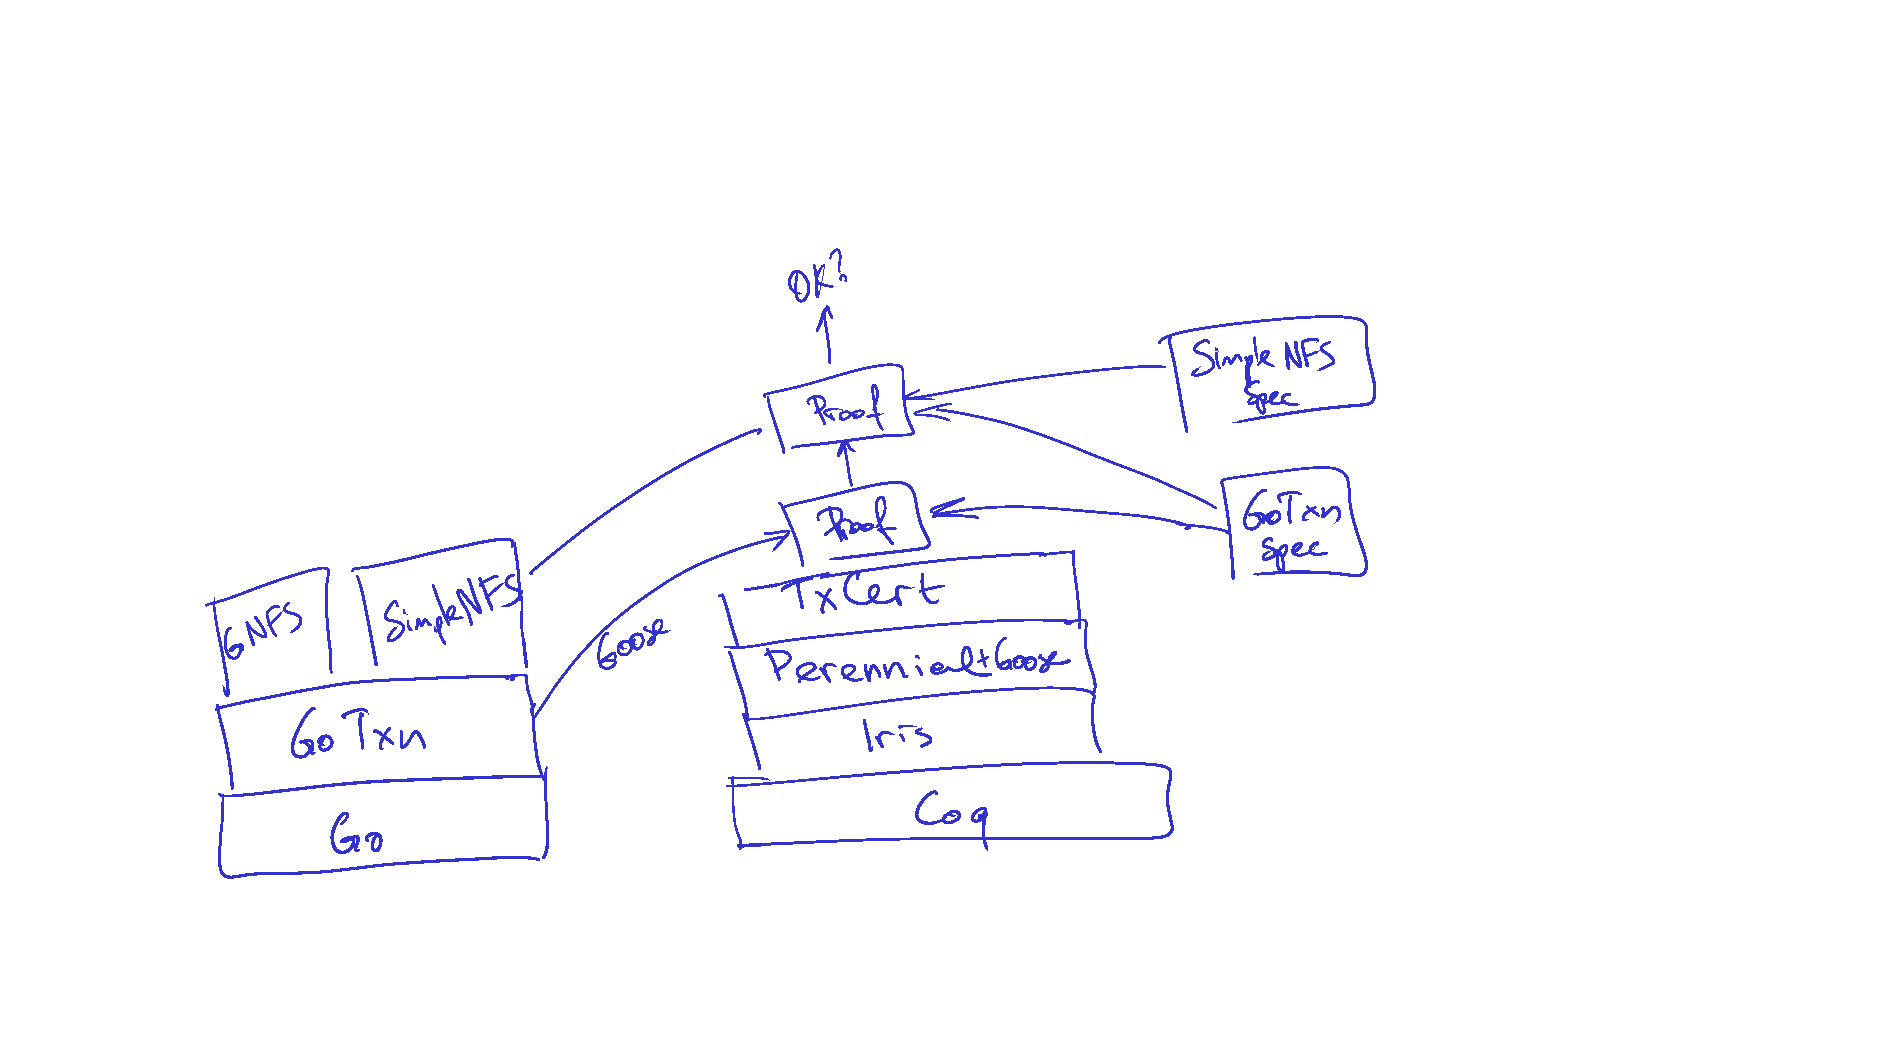
\includegraphics[width=\columnwidth]{fig/overview}
% \includegraphics{drawn-diagrams/jrnl-overview.png}
% \caption{Overview of Perennial, \txn, \simplenfs, and \gnfs.}
% \label{fig:overview}
% \end{figure}

\begin{figure}
\begin{tikzpicture}[>=latex, node distance=.5cm]

  \tikzstyle{other}=[fill=gray!20];

  \tikzstyle{layer}=[thick,rectangle, draw,minimum width=3.65cm,minimum
    height=.5cm, align=center];
  \tikzstyle{layerthin}=[outer sep=0, thick,rectangle, draw,minimum width=3.65cm,minimum
    height=.5cm, align=center];

  \tikzstyle{layermini}=[thick,rectangle, draw, minimum width=1.5cm,minimum height=.5cm,align=center];
  \tikzstyle{layerhalf}=[thick,rectangle, draw, minimum width=1.95cm,minimum height=.5cm,align=center];
  \tikzstyle{layeroverhalf}=[thick,rectangle, draw, minimum width=2.25cm,minimum height=.5cm,align=center];

  \tikzstyle{layers}=[thick,rectangle, draw, minimum
    width=1.75cm,minimum height=1cm,align=center];

  \tikzstyle{edge}=[->,thick];
  
  \draw node (coq) [layerthin, other] {Iris + Coq};
  %\draw node (iris) [layer, other,above of=coq] {Iris};
  %\draw node (goose) [layer, other, above of=iris] {Perennial + Goose};
  \draw node (jrnlcert) [layerthin, above of=coq] {Perennial 2.0};

  \draw node (go) [layerthin, other, left=1cm of jrnlcert] {Go};
  \draw node (gojrnl) [layer, above of=go] {\txn};
  \draw node (gnfs) [layermini, above=of gojrnl.west,anchor=west] {\gnfs};
  \draw node (simplenfs) [layerhalf, above=of gojrnl.east,anchor=east] {\simplenfs};
  \draw node (recexamp) [layerhalf, above of=simplenfs, font=\footnotesize] {Toy Client};

  \draw node (gojrnlspec) [layeroverhalf, above=.75cm of jrnlcert.east,anchor=east, font=\footnotesize] {\txn Spec};
  \draw node (simplenfsspec) [layeroverhalf, above of=gojrnlspec, font=\footnotesize] {\simplenfs Spec};
  \draw node (recspec) [layeroverhalf, above of=simplenfsspec, font=\footnotesize] {Example Spec};


  \tikzstyle{proofnode}=[dashed,rectangle, draw, minimum width=1.25cm,minimum height=.5cm,align=center];
  \draw node (proof1) [proofnode, above=0cm of jrnlcert.north west,anchor=south west] {Proof};
  \draw node (proof2) [proofnode, above of=proof1] {Proof};
  \draw node (proof3) [proofnode, above of=proof2] {Proof};

  \draw node (bin) [above=2.15cm of gojrnl] {\cc{a.out}};
  \draw [edge] (gojrnl.north)+(0,1.25cm) -- node[left] {\cc{go build}} (bin.south);

  \draw [edge, shorten >=.15cm, shorten <=.15cm] (gojrnl) -- (proof1);
  \draw [edge, shorten >=.15cm, shorten <=.15cm] (simplenfs) -- (proof2);
  \draw [edge, shorten >=.15cm, shorten <=.15cm] (recexamp) -- node[above] {Goose} (proof3);

  \path let \p1=(bin) in let \p2=(proof3) in node (ok) at (\x2, \y1) {OK?};
  \draw [edge, transform canvas={xshift=3.45cm}] (gojrnl.north)+(0,1.25cm) -- (bin.south);
  %\draw [edge, shorten >=.15cm, shorten <=.15cm] (proof3) -- node[right] {{\tt coqc}} (ok);

  %{\cc{go build}};
  % \draw node (coqgo) [layerm,above=of goose,anchor=north] {Coq
  %   representation of Go (\cref{ch:goose})};
  % \draw node (perennial) [layerm,above=of iris.east,anchor=east] {\sys library
  %   for\\concurrency and recovery (\cref{ch:proving})};
  % \draw node (proof) [layers,above=of perennial.west,anchor=west,fill=green!10,dashed] {Proof};
  % \draw node (spec) [layers,above= of perennial.east,anchor=east,fill=green!10,dashed] {Spec};

  % \draw node (code) [layers,left of=coqgo,node distance=5cm,fill=green!10,dashed] {Go src};
  % \draw node (bin) [layers,below=of code] {a.out};
  % \draw [edge] (code.south) -- node[right] {Go compiler} (bin.north);

  % \draw [edge] (code.east) -- node[above] {Goose} node[below] {Translator} (coqgo.west);
  % \draw [edge] (coqgo.east) -- (proof.west);
  % \draw [edge] (spec.west) -- (proof.east);

  % \draw [edge] (proof.north) -- node[above] {OK?} ($(proof.north)+(0.0,+0.3)$);
          
\end{tikzpicture}

\caption{Overview of Perennial, \txn, \simplenfs, and \gnfs.}
\label{fig:overview}
\end{figure}

\autoref{fig:overview} gives an overview of how \txn and systems
building on it are verified using Perennial.
On the left of the figure is the executable code, which is written
in Go. On top of \txn, we have implemented two NFS servers to evaluate \txn
along different dimensions. \gnfs is a functional NFS server that is sufficient
to run real applications, which we use to assess \txn's scalability and
performance. Meanwhile, \simplenfs is a verified, core subset of \gnfs's
functionality, which evaluates the usability of \txn's specs for building
verified systems on top of it.
% \gnfs supports most of RFC 1813~\cite{RFC:1813}, with
% the exception of symbolic links and permissions.  \gnfs supports the
% \cc{unstable} argument to the write RPC, allowing for writes that are
% not immediately flushed to disk, as well as the commit RPC that flushes
% these writes.  To allow this, \txn supports transactions that commit
% but are not immediately flushed to disk.  To formally validate the
% specifications of \txn, we verified \simplenfs, a core subset of \gnfs.

On the right side of the figure is the verification stack. The verification
builds on the Perennial 2.0 framework, which is itself implemented in the Iris
framework in the Coq proof assistant. To reason about executable code, a tool
called Goose translates a Go implementation into a model that we can prove
specifications about in Perennial. Perennial provides a model of execution for
Go code that incorporates crash-safety and concurrency, which
includes a model of the disk (with atomic, synchronous reads and writes of 4KB
sectors) as well as a model of crashes and recovery (crashes at arbitrary points
during execution, and jumping to specific boot code for recovery after a crash).

\txn's top-level specification describes its API in terms of an extension of
concurrent separation logic, with pre-, post-, and crash conditions. These
specifications capture the behavior of individual Go functions: if the function
is run in a state satisfying its precondition, then the final state will satisfy
the postcondition, and if the system crashes the state will satisfy the crash
condition. The specification for the journaling API is described in detail in \autoref{s:design}. We
demonstrate the usefulness of this specification by proving correctness of the \simplenfs
server using logically atomic crash specifications (\autoref{s:proof:logatom}). %, a style of specification
%encoded in Hoare triples.
The top-level theorem for \simplenfs states that its RPCs
atomically follow transitions of a state machine formalizing the NFSv3 protocol (based on RFC
1813~\cite{RFC:1813}).

As described in FSCQ and Argosy~\cite{chen:fscq,chajed:argosy}, crash conditions
can be used to reason about recovery procedures, even crashes during recovery. A
recovery procedure can safely be re-run after a crash if its specification is
\emph{idempotent}: its crash condition should imply its precondition. As an
end-to-end check of the crash specs in \simplenfs and \txn, showing they support
recovery correctly, we prove an idempotent specification for a toy example
client on top of \simplenfs, establishing that it can successfully execute even if
\simplenfs crashes and recovers an arbitrary number of times.

The proof of \txn's specification depends on a number of assumptions. We assume
that the disk writes 4KB blocks atomically, even on crash, and assume that the
code executes according to the Perennial model generated by Goose. The
specification relies on the caller to provide concurrency control; the proof of
\simplenfs checks that locking is performed correctly, but \gnfs is unverified
and we trust that its concurrency control is correct in order to make operations
atomic (though this does not say they correctly implement the NFS
specification).

% \begin{figure}[ht]
%   \begin{Verbatim}[commandchars=\\\{\},codes={\catcode`\$=3\catcode`\^=7\catcode`\_=8},fontsize=\small]
\PY{c}{(*}\PY{c}{ The state of SimpleNFS is a map from file handles}
\PY{c}{(}\PY{c}{inode numbers}\PY{c}{)}\PY{c}{ to contents }\PY{c}{(}\PY{c}{list of bytes}\PY{c}{)}\PY{c}{. }\PY{c}{*)}
\PY{k+kn}{Definition} \PY{n}{State} \PY{o}{:=} \PY{n}{gmap} \PY{n}{fh} \PY{o}{(}\PY{n}{list} \PY{n}{u8}\PY{o}{)}\PY{o}{.}

\PY{k+kn}{Definition} \PY{n}{write} \PY{o}{(}\PY{n}{f} \PY{o}{:} \PY{n}{fh}\PY{o}{)} \PY{o}{(}\PY{n}{off} \PY{o}{:} \PY{n}{u64}\PY{o}{)}
           \PY{o}{(}\PY{n}{d} \PY{o}{:} \PY{n}{list} \PY{n}{u8}\PY{o}{)} \PY{o}{(}\PY{n}{d0} \PY{o}{:} \PY{n}{list} \PY{n}{u8}\PY{o}{)}
    \PY{o}{:} \PY{n}{transition} \PY{n}{State} \PY{n}{u32} \PY{o}{:=}
  \PY{c}{(*}\PY{c}{ Convert u64 to mathematical integer }\PY{c}{*)}
  \PY{k}{let} \PY{n}{off} \PY{o}{:=} \PY{n}{int}\PY{o}{.}\PY{n}{nat} \PY{n}{off} \PY{k}{in}
  \PY{c}{(*}\PY{c}{ Simplified spec does not allow creating holes,}
\PY{c}{     but does allow appending }\PY{c}{*)}
  \PY{n}{check} \PY{o}{(}\PY{n}{off} ≤ \PY{n}{length} \PY{n}{d0}\PY{o}{)}\PY{o}{;}
  \PY{k}{let} \PY{n}{d\PYZsq{}} \PY{o}{:=} \PY{n}{d0}\PY{o}{[}\PY{o}{:}\PY{n}{off}\PY{o}{]} \PY{o}{+}\PY{o}{+} \PY{n}{d} \PY{o}{+}\PY{o}{+} \PY{n}{d0}\PY{o}{[}\PY{n}{off}\PY{o}{+}\PY{n}{length} \PY{n}{d}\PY{o}{:}\PY{o}{]} \PY{k}{in}
  \PY{c}{(*}\PY{c}{ Update spec file state }\PY{c}{*)}
  \PY{n}{modify} \PY{o}{(}\PY{k}{fun} \PY{n}{s} \PY{o}{=\PYZgt{}} \PY{n}{insert} \PY{n}{f} \PY{n}{d\PYZsq{}} \PY{n}{s}\PY{o}{)}\PY{o}{;}
  \PY{n}{ret} \PY{o}{(}\PY{n}{U32} \PY{o}{(}\PY{n}{length} \PY{n}{d}\PY{o}{)}\PY{o}{)}\PY{o}{.}
\end{Verbatim}

%   \vspace{-\baselineskip}
%   \caption{Specification for an NFS \textsc{write} which writes \cc{d} to
% file handle \cc{f} at offset \cc{off}. A wrapper around the spec checks that
% \cc{f} is a valid handle, passes the current file contents \cc{d0}, and allows
% the spec to return an error (e.g., if out of disk space). }
%   \label{fig:nfswritespec}
% \end{figure}
%
% \joe{We should probably trim this down now, since we don't much care about SimpleNFS's TCB anymore. Maybe rephrase it in terms of GoJournal's tcb?}
% The end-to-end proof for an application using \txn, such as \simplenfs, depends on a number of assumptions.
% The proof itself relies on the Coq proof assistant being correct, and
% on the top-level specification of \simplenfs correctly capturing its
% intended behavior.  The proof also relies on Goose to faithfully model
% the Go code of \simplenfs and \txn in Coq, and on the Go compiler and
% runtime to correctly execute the code.  The proof also assumes that the
% disk model is accurate (atomic and synchronous sector writes).  Finally,
% the proof does not cover the code that parses XDR-encoded RPC requests.
% We use a separate tool to generate this Go code from an XDR description
% of the protocols~\cite{RFC:1813, RFC:1057, RFC:4506}.

